\chapter{Diseño}

\section{Arquitectura Software}

La arquitectura software se refiere a la estructura o estructuras de un sistema software, que comprenden componentes de software, sus propiedades visibles externamente y las relaciones entre ellos. Es una disciplina esencial en la ingeniería de software que aborda la organización de un sistema como una composición de componentes, los protocolos de comunicación y sincronización, y la asignación de funciones a elementos de diseño. Una buena arquitectura de software garantiza que un sistema cumpla con requisitos clave como rendimiento, fiabilidad, portabilidad, escalabilidad e interoperabilidad, y sirve como un puente crítico entre los requisitos del sistema y el código implementado. [REF]

Para el desarrollo de la aplicación móvil, se ha optado por una arquitectura cliente-servidor basada en una arquitectura orientada a servicios (SOA) debido a su capacidad para facilitar la comunicación entre el servidor y la aplicación móvil. La API, desarrollada en Python y Flask, maneja las solicitudes del cliente. Los usuarios realizan peticiones desde la aplicación móvil al servidor, y este responde con la información solicitada, Esta arquitectura permite una interacción eficiente entre el cliente y el servidor, asegurando una experiencia de usuario fluida.


\subsection{Arquitectura Orientada a Servicios}

La Arquitectura Orientada a Servicios (SOA) es un paradigma que organiza capacidades distribuidas en la red, haciendo visibles los servicios a los usuarios y permitiendo la interacción mediante intercambios de información para producir efectos reales. La llamada a servicios se basa en lenguajes y protocolos estándar, facilitando interoperabilidad y presentando las operaciones como atómicas desde la perspectiva del usuario. SOA permite soluciones flexibles, escalables y eficientes, liberando a los usuarios para concentrarse en la usabilidad sin preocuparse por los detalles técnicos internos. [REF]

En el contexto de una arquitectura cliente-servidor, las llamadas a los servicios se realizan mediante llamadas HTTP, y la información se devuelve en formato JSON, que es el estándar para la intercomunicación en esta arquitectura. Este enfoque asegura una comunicación clara y estructurada entre el cliente y el servidor, permitiendo un manejo eficiente de los datos.

\begin{figure}[H]
    \centering
    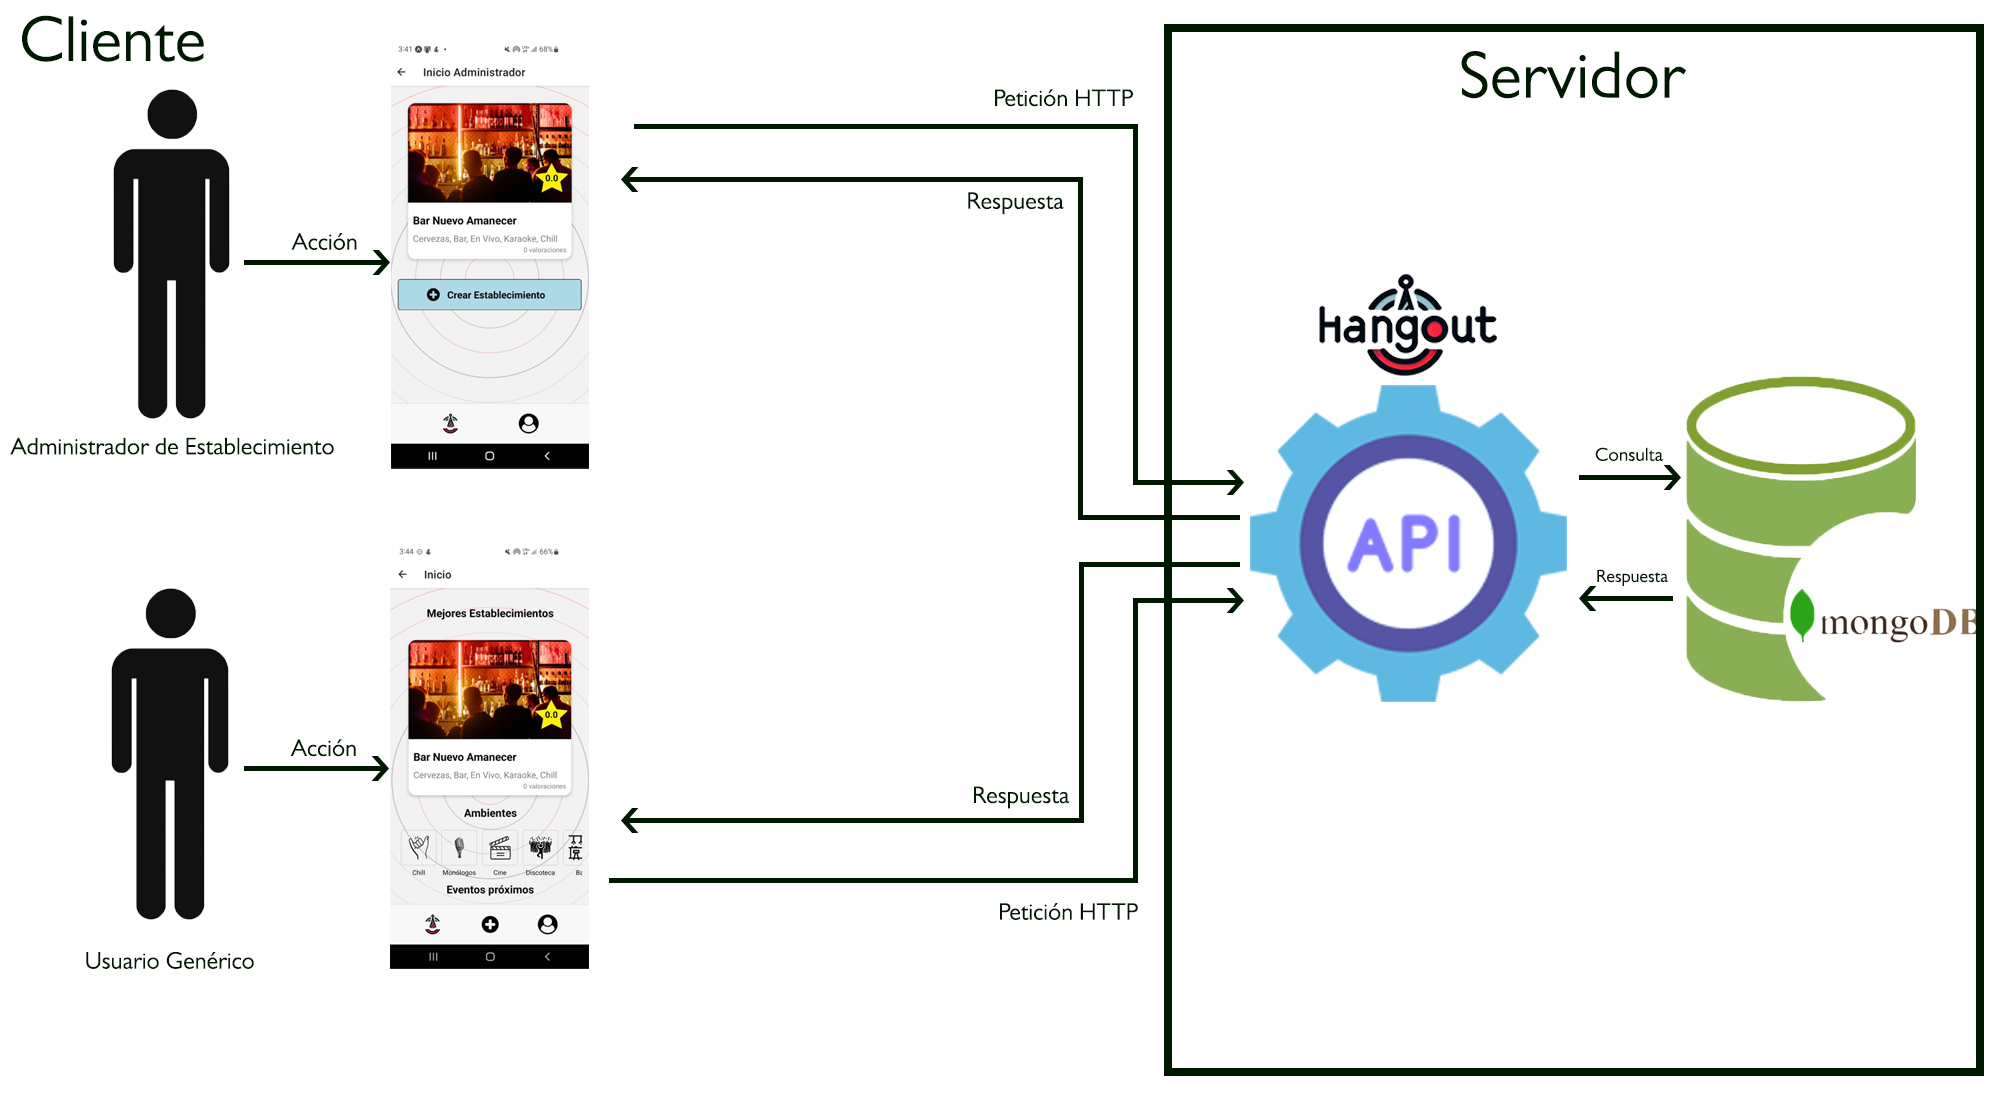
\includegraphics[width=\textwidth]{imagenes/ARQUITECTURA.jpg}
    \caption{Arquitectura Orientada a Servicios basada en Cliente-Servidor}
    \label{fig:ARQUITECTURA}
\end{figure}


\section{Tecnologías Utilizadas}

Para el desarrollo de la aplicación móvil, se necesita tanto un backend como un frontend. El backend funciona como un servidor al que se hacen las peticiones, implementado mediante una API en Python con Flask y utilizando MongoDB como base de datos. El frontend incluye la interfaz de usuario, desarrollada en React Native, desde donde los usuarios interactúan y realizan las llamadas a la API. En las secciones siguientes se detallarán estas implementaciones con mayor profundidad.

\subsection{Desarrollo Backend}

\textbf{Python 3.12.3:} Es un lenguaje de programación interpretado, orientado a objetos y de alto nivel con semántica dinámica. Sus estructuras de datos de alto nivel incorporadas, combinadas con la tipificación dinámica y el enlace dinámico, lo hacen muy atractivo para el desarrollo rápido de aplicaciones, así como para su uso como lenguaje de script o "pegamento" para conectar componentes existentes. La sintaxis simple y fácil de aprender de Python enfatiza la legibilidad y, por lo tanto, reduce el costo de mantenimiento del programa. Python soporta módulos y paquetes, lo que fomenta la modularidad del programa y la reutilización del código. [REF]

La elección de utilizar Python para el desarrollo del backend fue una recomendación de mi tutor. Además, aprender uno de los lenguajes de programación más utilizados a nivel mundial fue una motivación adicional. Python es reconocido por su facilidad de aprendizaje y su sintaxis clara y directa, esto lo convierte en una opción ideal si ya se tiene experiencia en otros lenguajes. En mi caso, el conocimiento previo de Ruby, que posee algunas similitudes con Python, hizo que la transición  y el aprendizaje resultara más sencillo.

\textbf{Flask 3.0.2:} Es un microframework para Python que facilita la creación de las API. Fue diseñado para ser sencillo y fácil de usar, permitiendo a los desarrolladores construir aplicaciones rápidamente con una mínima configuración. Flask es conocido por su flexibilidad y modularidad, lo que permite a los desarrolladores elegir las herramientas y bibliotecas que mejor se adapten a sus necesidades. [REF]

El uso de Flask, además de ser una recomendación de mi tutor, se debió a la excelente documentación disponible sobre este framework. Las guías detallan desde la configuración inicial hasta los aspectos que pueden resultar más complejos, proporcionando indicaciones y ejemplos. Necesitaba un framework que además de tener una curva de aprendizaje sencilla, facilitara la conexión a bases de datos, y con la biblioteca \texttt{flask\_pymongo} hizo que todo resultara más simple.


\textbf{MongoDB 7.0.7:} MongoDB es una base de datos de documentos que proporciona escalabilidad y flexibilidad, permitiendo almacenar datos en documentos similares a JSON. Esto facilita la variación y evolución de la estructura de datos con el tiempo. Ofrece consultas ad hoc, indexación avanzada y agregación en tiempo real. MongoDB está diseñado como una base de datos distribuida, asegurando alta disponibilidad y escalabilidad horizontal, siendo adecuado para aplicaciones modernas que requieren flexibilidad y rendimiento. [REF]

El empleo de MongoDB se debe a las razones mencionadas anteriormente, ya que ofrece la biblioteca \texttt{flask\_pymongo} que facilita la comunicación entre el framework y la base de datos. Además, como la descripción de MongoDB indica este permite el almacenamiento de datos en documentos similares a JSON, lo cual es lo ideal para las necesidades de la aplicación, ya que se buscaba una forma flexible y eficiente de gestionar la información. 

\subsection{Desarrollo Frontend}

\textbf{Node.js 20.12.2:} Es un entorno de ejecución de JavaScript asíncrono y basado en eventos, diseñado para crear aplicaciones de red escalables. Permite manejar múltiples conexiones simultáneas sin bloquear el proceso, lo que lo hace eficiente y adecuado para el desarrollo de sistemas escalables. Node.js toma el modelo de eventos un poco más allá, presentando un bucle de eventos como una construcción de tiempo de ejecución en lugar de una biblioteca. [REF]

El uso de Node.js es un requisito para utilizar React Native con Expo debido que este proporciona el entorno de ejecución necesario para las herramientas de desarrollo de JavaScript

\textbf{Java Development Kit 17.0.10:} Es un paquete de software necesario para el desarrollo de aplicaciones en Java. Incluye el JRE (Java Runtime Environment), que permite ejecutar programas Java. [REF]

Este es otro requerimiento para el uso de React Native con Expo debido a que proporciona las herramientas necesarias para la compilación y ejecución del código para aplicaciones Android ya que estas se construyen con Java en su parte nativa.

\textbf{React Native 0.74.1:} React Native es un framework de desarrollo de aplicaciones móviles que permite crear aplicaciones nativas para Android y iOS y otras plataformas utilizando React y JavaScript. Desarrollado por Facebook, React Native combina lo mejor de React con las capacidades nativas, permitiendo a los desarrolladores escribir una vez y ejecutar en cualquier lugar. Hace uso de componentes nativos como puede ser View, Text e Image que se traducen en bloques de construcción de la interfaz de usuario nativa de la plataforma, proporcionando un rendimiento y experiencia de usuario nativos. Esto permite crear el FrontEnd y desplegarlo tanto en la App Store de Apple como en la Play Store de Google. De allí su lema “Learn Once Write Anywhere” [REF]

La utilización de React Native se basa principalmente en que consideré que sería la opción segura y sencilla para el desarrollo de una aplicación móvil, permitiendo escribir el código en un único formato y generar tanto el APK para Android como el archivo para iOS. La utilización de los componentes anteriormente mencionados facilita la lectura y mejora la experiencia de desarrollo. Además, React Native permite una alta reutilización de código gracias a la creación de componentes propios y reutilizables. 

Un aspecto importante en mi decisión fue la disponibilidad de Expo, una herramienta que simplifica la configuración inicial, especialmente para aquellos que nunca han trabajado con React o React Native, permitiendo visualizar los cambios en tiempo real en una aplicación móvil.

\subsection{Herramientas de Desarrollo}

\textbf{Visual Studio Code 1.90.0:} Es un editor de código fuente ligero pero potente, desarrollado por Microsoft. Está disponible para Windows, macOS y Linux, y se utiliza para escribir, depurar y editar código. Ofrece características como resaltado de sintaxis, autocompletado de código, integración con Git, y un grupo de extensiones que permite personalizar y ampliar su funcionalidad para soportar una amplia gama de lenguajes de programación y flujos de trabajo de desarrollo. [REF]

La principal razón de la elección de Visual Studio Code ha sido mi familiaridad con él, ya que lo he estado utilizando desde los inicios del grado. Sus extensiones facilitan en gran medida la programación. Además, como mencioné en la descripción, la funcionalidad de autocompletado lo convierte en una de las mejores opciones. También permite integrar terminales para ejecutar los comandos desde el mismo entorno, lo cual mejora la eficiencia a la hora de trabajar.

\textbf{Android Studio 2023.3.1:} Es el entorno de desarrollo integrado oficial para el desarrollo de aplicaciones Android. Ofrece herramientas avanzadas de edición de código, depuración, pruebas y rendimiento, y está diseñado para acelerar el desarrollo y la calidad de las aplicaciones Android.

Solo ha sido necesario utilizar Android Studio en el proyecto para ejecutar el emulador de Android y realizar pruebas en él, además de las pruebas que ya se realizaban en la aplicación Expo Go desde mi propio móvil.

\textbf{Postman 10.24:}  Postman es una plataforma de colaboración para el desarrollo de APIs que simplifica cada etapa del ciclo de vida de las API, desde el diseño y la prueba hasta la implementación y el monitoreo. Permite a los desarrolladores enviar solicitudes HTTP, crear y ejecutar pruebas automatizadas, y documentar la API de manera más eficiente. [REF]

Ha sido uno de los pilares fundamentales para el desarrollo de mi aplicación móvil especialmente en el backend ya que desde esta aplicación podía comprobar el correcto funcionamiento de los endpoints comprobando si al envíar una solicitud se devolvía una respuesta esperada. También ha sido crucial para el desarrollo del frontend, ya que desde esta herramienta he podido depurar errores y entender el porqué de las respuestas API no no devolvían lo esperado. Esto facilitó la identificación y corrección de problemas en las solicitudes y respuestas HTTP durante el desarrollo.

\section{Modelo de Datos}

Para la base de datos se ha utilizado MongoDB. Su estructura NoSQL basada en documentos JSON facilita la comunicación entre el cliente y el servidor, haciendo que el manejo de datos sea más flexible y eficiente. Dado que el diagrama de clases muestra todas las clases, cada una de estas se traduce en una colección, donde sus campos son los atributos de clase. Esto se verá con mayor claridad en el Diagrama de Clases, proporcionando una visión estructurada y comprensible de la organización de los datos.

\section{Diseño Lógico}

Los diagramas de clase UML modelan la estructura estática de un dominio de aplicación en términos de clases y relaciones entre ellas. Estos diagramas son esenciales en el diseño lógico software, ya que permiten visualizar y documentar entidades y sus interacciones, asegurando consistencia y cumplimiento de los requisitos. [REF]

Para definir la elaboración del diseño lógico del sistema se ha optado por crear el siguiente diagrama de clases

\begin{figure}[H]
    \centering
    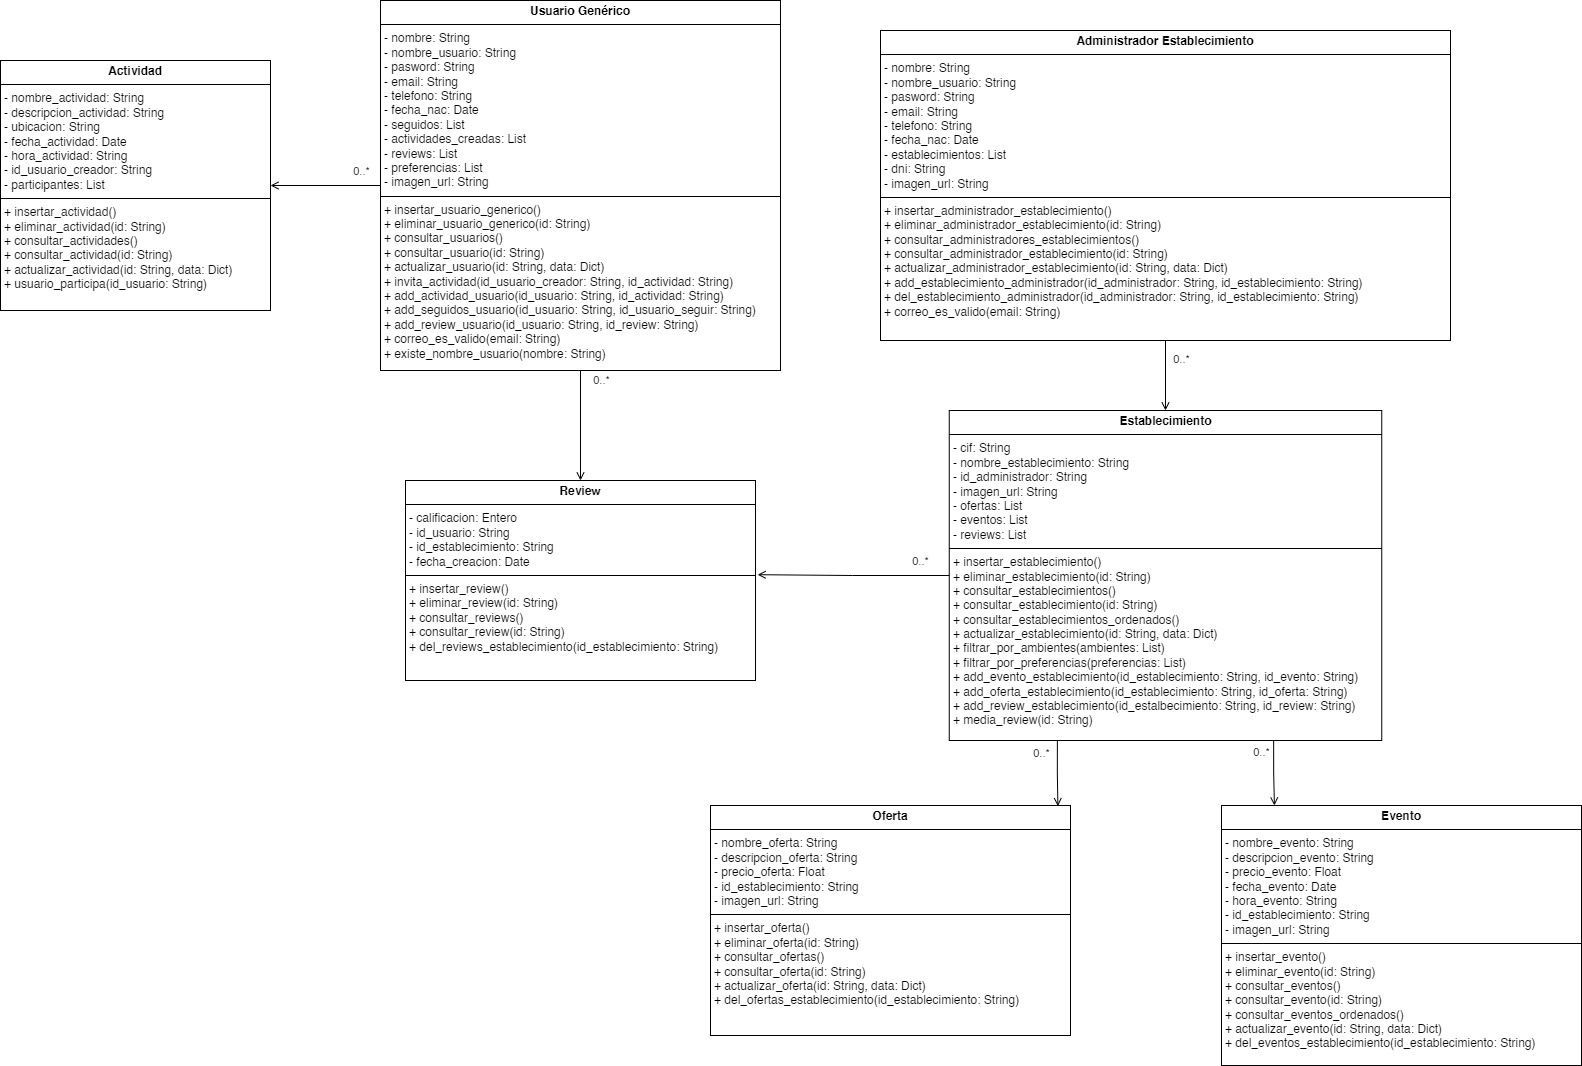
\includegraphics[width=\textwidth]{imagenes/DiagramaHangOut.jpg}
    \caption{Diagrama de clases de la aplicación desarrollada}
    \label{fig:DiagramaHangOut}
\end{figure}


\section{Diseño de MockUps para Frontend}

El diseño de mockups para el frontend es una parte importante para el desarrollo de la interfaz de usuario de la aplicación. Los mockups son representaciones visuales de la interfaz que muestra cómo se verán las páginas y componentes de la aplicación antes de su implementación. Estos diseños ayudan a planificar la estructura y la navegación, asegurando una experiencia de usuario intuitiva y agradable. 

Para la elaboración de estos mockups me inspiré en un diseño de aplicación disponible en Behance. El diseño específico en el cual basé el diseño se titula “Eventify - Event and Party App Case Study”[REF]. A continuación se presentan algunos mockups que utilicé para el diseño del frontend los cuales sirvieron de base para la creación de la interfaz de usuario.

\clearpage
\vspace*{\fill}
\begin{figure}[H]
    \centering
    \begin{subfigure}{0.45\textwidth}
        \centering
        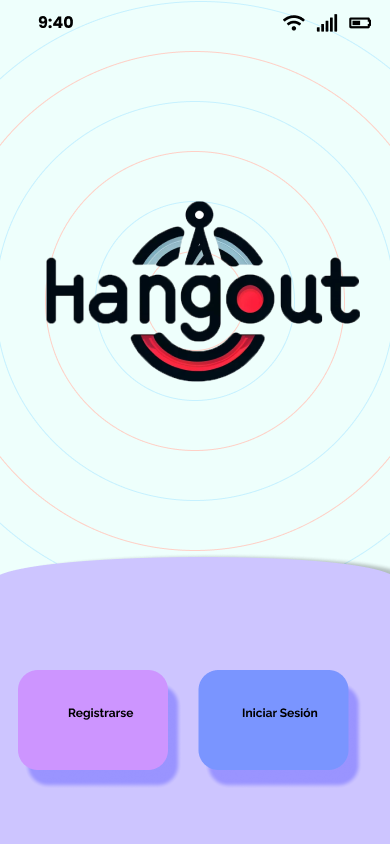
\includegraphics[width=\linewidth]{imagenes/mockup1.png}
        \caption{Inicio de aplicación}
        \label{fig:img1}
    \end{subfigure}%
    \hfill
    \begin{subfigure}{0.45\textwidth}
        \centering
        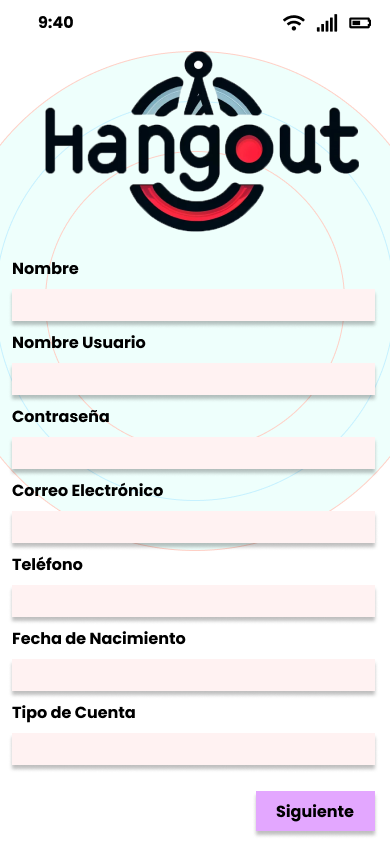
\includegraphics[width=\linewidth]{imagenes/mockup2.png}
        \caption{Formularios de la aplicación}
        \label{fig:img2}
    \end{subfigure}
\end{figure}
\vspace*{\fill}

\clearpage
\vspace*{\fill}
\begin{figure}[H]
    \centering
    \begin{subfigure}{0.45\textwidth}
        \centering
        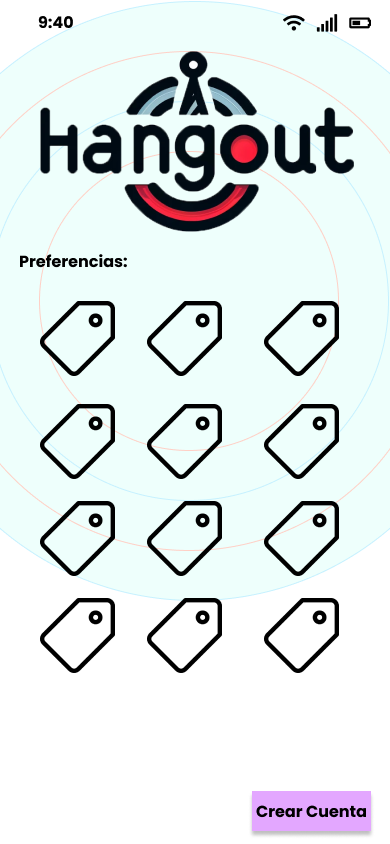
\includegraphics[width=\linewidth]{imagenes/mockup3.png}
        \caption{Selección de preferencias}
        \label{fig:img3}
    \end{subfigure}%
    \hfill
    \begin{subfigure}{0.45\textwidth}
        \centering
        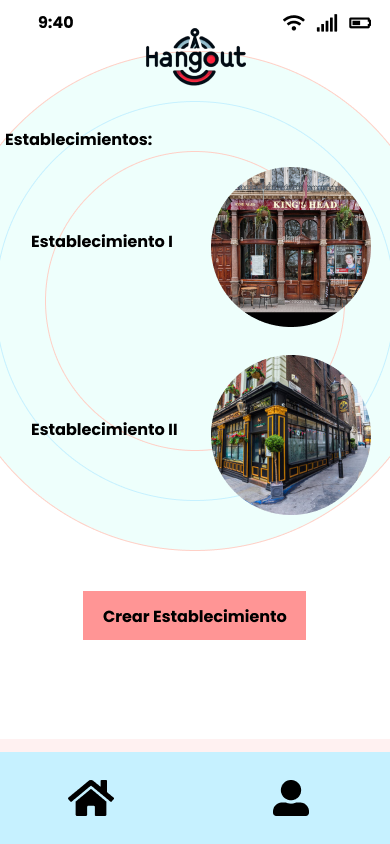
\includegraphics[width=\linewidth]{imagenes/mockup4.png}
        \caption{Inicio de Administrador de Establecimiento}
        \label{fig:img4}
    \end{subfigure}
\end{figure}
\vspace*{\fill}

\clearpage
\vspace*{\fill}
\begin{figure}[H]
    \centering
    \begin{subfigure}{0.45\textwidth}
        \centering
        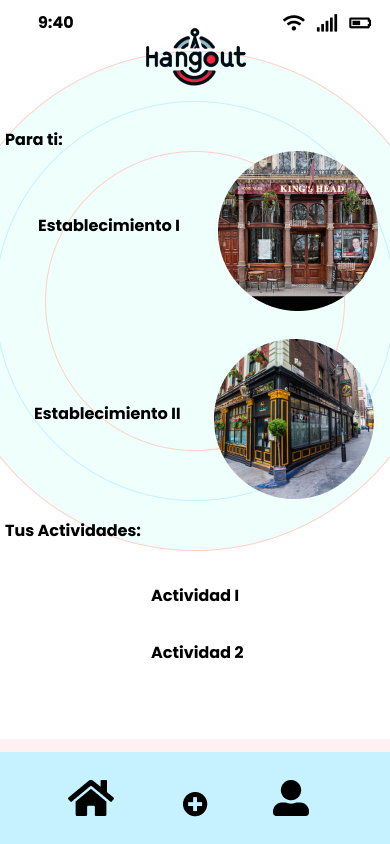
\includegraphics[width=\linewidth]{imagenes/mockup5.png}
        \caption{Inicio de Usuario Genérico}
        \label{fig:img5}
    \end{subfigure}%
    \hfill
    \begin{subfigure}{0.45\textwidth}
        \centering
        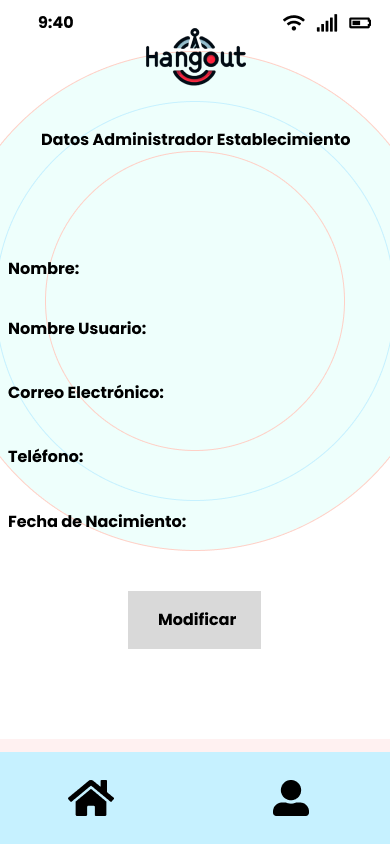
\includegraphics[width=\linewidth]{imagenes/mockup6.png}
        \caption{Muestra de Datos}
        \label{fig:img6}
    \end{subfigure}
\end{figure}
\vspace*{\fill}